\documentclass[10pt, conference, letterpaper]{IEEEtran}

\usepackage{algorithm}
\usepackage{algorithmicx}
\usepackage{algpseudocode}
\usepackage{amsfonts}
\usepackage{amsmath}
\usepackage{amssymb}
\usepackage[ansinew]{inputenc}
%\usepackage{xcolor}
\usepackage[table,xcdraw]{xcolor}
\usepackage{mathtools}
\usepackage{graphicx}
\usepackage{caption}
\usepackage{subcaption}
\usepackage{import}
\usepackage{multirow}
\usepackage{cite}
\usepackage[export]{adjustbox}
\usepackage{breqn}
\usepackage{mathrsfs}
\usepackage{acronym}
\usepackage[keeplastbox]{flushend}
\usepackage{setspace}
\usepackage{stackengine}
\usepackage{wrapfig}

\renewcommand{\thetable}{\arabic{table}}
\renewcommand{\thesubtable}{\alph{subtable}}

\DeclareMathOperator*{\argmin}{arg\,min}
\DeclareMathOperator*{\argmax}{arg\,max}

\def\delequal{\mathrel{\ensurestackMath{\stackon[1pt]{=}{\scriptscriptstyle\Delta}}}}

\graphicspath{{./figures/}}
\setlength{\belowcaptionskip}{0mm}
\setlength{\textfloatsep}{8pt}

\newcommand{\eq}[1]{Eq.~\eqref{#1}}
\newcommand{\fig}[1]{Fig.~\ref{#1}}
\newcommand{\tab}[1]{Tab.~\ref{#1}}
\newcommand{\secref}[1]{Section~\ref{#1}}

\newcommand\MR[1]{\textcolor{blue}{#1}}
\newcommand\red[1]{\textcolor{red}{#1}}

%\renewcommand{\baselinestretch}{0.98}
% \renewcommand{\bottomfraction}{0.8}
% \setlength{\abovecaptionskip}{0pt}
\setlength{\columnsep}{0.2in}

% \IEEEoverridecommandlockouts\IEEEpubid{\makebox[\columnwidth]{PUT COPYRIGHT NOTICE HERE \hfill} \hspace{\columnsep}\makebox[\columnwidth]{ }} 

\title{Human Activity Recognition: a comparison of different convolutional neural network architectures}

\author{Damnko$^\dag$
\thanks{$^\dag$Name Surname: email-address}
}

\IEEEoverridecommandlockouts

\begin{document}

\maketitle

\begin{abstract}
Human body motion analysis based on wearable inertial measurement units (IMUs) has been receiving a lot of attention in recent years. This is due to the significant role in both the scientific and industrial communities, with uses that span from mobile health systems to sports and human computer interaction. Human Activity Recognition (HAR) system with high recognition accuracy using only a single sensor is still a technical challenge. In this paper I explore both supervised and partially supervised approaches using convolutional, deep convolutional and denoising autoencoders approaches. The goal of this paper is to enhance on the classification accuracy of previous related works and decrease reliance on human engineered features. Since the raw IMU data is composed of time series, it is split using a running window approach and segments of roughly one second of data are fed to the neural networks. The above approaches are tested with two different variations of the original dataset, obtained with data augmentation approaches, to compensate the disparity in the representation of the different classes. The dataset contains measurements of one single IMU sensor positioned in the belt of different users performing 7 actions: \textit{\textbf{running, jumping, walking, falling, sitting, standing, lying}}. The results show that the best \mbox{CNN-based} HAR system achieved an \mbox{F1-Score} of 0.972. The worst represented class, falling, with just 4 minutes of recorded data, has an F1-Score of 0.919.
\end{abstract}

\IEEEkeywords
Neural networks, machine learning, denoising autoencoders, convolutional neural network, human activity recognition, inertial sensors
\endIEEEkeywords


% !TEX root = template.tex

\section{Introduction}
\label{sec:introduction}

In recent years, there has been substancial effort on employing wearable devices for HAR. Due to their small size, portability, and high processing power, IMUs are widely used for complex motion analysis: usage in sports training, videogames, as well as medical applications such as analysis of patients' health based on gait abnormalities and fall detection \cite{Yamada-2012}, smart assistive technologies, such as in smart homes \cite{Parisa-2009}, in rehabilitation \cite{Shyamal-2012}, in health support \cite{Akin-2010}, in skill assessment \cite{Matthias-2013} and in industrial settings \cite{Thomas-2008}.
HAR has been studied by using computer vision approaches \cite{Hueihan-2013,Ferda-2013}, IMUs approaches \cite{jian-2015,nils-2016,Valarezo-2017} and hybrid approaches using data from both inertial sensors and cameras \cite{2017-mfi-actionrecognition}.
\mbox{On-body} sensors enjoy the merits of information privacy: the signals they acquire are target specific and do not reveal any personal information on the specific user nor other nontarget subjects in the scene. Moreover, this allows activity recognition regardless of the location of the user, which wouldn't be possible in a \mbox{fixed-camera} setup.
A typical HAR system is composed of two key elements: one or more smart sensors and a pattern recognition system. With IMUs, human movements are translated into time series information of acceleration via accelerometer and angles via gyroscope. Although multiple sensors can be used in order to improve the accuracy of the method, as in \cite{Grzezick-2017}, this approach is less practical due to the more elaborate setup. This study focuses on classifying activities using data recorded by a single IMU sensor placed on the belt of the subjects. \par
The goal of this paper is twofold: to improve the classification accuracy of previous related works and decrease reliance on human engineered features in order to address increasingly complex recognition problems.
HAR approaches with manual feature extraction \cite{base-paper} as well as automatic \cite{jian-2015, nils-2016, Valarezo-2017} have already been proposed, however none of them succed in describing and comparing in a systematic and detailed way the training process for deep, convolutional, and stacked convolutional autoencoder models. \par
Implementing an effective HAR system using only a single sensor is still a technical challenge. For this reason I experimented with different machine learning approaches: convolutional neural networks (CNNs), deep CNNs and stacked denoising autoencoders for classification of 7 activities.\\
A key aspect when using convolutions is whether to convolve only along the time dimension. This paper shows that best results are achieved when convolving first along the time dimension and then considering the cross correlation between multiple sensor data.
I also experimented with some data augmentation techniques, which gave an increased accuracy on underrepresented classes.\par

This paper contributes to the current research material:
\begin{itemize}
\item by exploring in depth novel techniques such as stacked denoising autoencoders and deep CNNs which has been gaining a lot of traction is numerous fields
\item by proposing effective and \mbox{non-handcrafted} features extraction techniques. These features also own more discriminative power, since the CNN can be trained under the supervision of output labels
\item by exploring two data augmentation techniques which can improve the classification accuracy of specific classes
\item by releasing the open source code, which can be used as starting point for future developments
\end{itemize}

The structure of this paper is organized as follows: \secref{sec:related_work} describes some related works. \secref{sec:processing_architecture} my proposed pipeline. \secref{sec:signals_features} the input data and signal processing, \secref{sec:learning_framework} present an in depth description of the learning framework. Finally, in \secref{sec:results}, the experimental results are presented.

% !TEX root = template.tex

\section{Related Work}
\label{sec:related_work}

In the past, HAR approaches were developed by following the standard pipeline in pattern recognition activities: segment extraction from an input time-series sequence, computing human engineered features and predicting class labels. Various modeling algorithms such as Support Vector Machine (SVM), Naive Bayes \cite{base-paper}, Random Forest or sequence based approaches such as Dynamic Time Warping \cite{Daniel-2015} or Hidden Markov Model \cite{Andreas-2014, Francisco-2014} were frequently used.

However, the performance of the aforementioned approaches is heavily dependant on the hand-crafted features. Extracting such features for machine learning systems is subjective, more error prone and can result in poor expressivity of the feature set.
In \cite{base-paper} the authors manually chose 19 features, derived from various sensor measures, which were carefully selected because of their discriminative power between the various activities that were tracked. Their work applies and compares different Bayesian estimation techniques. In most cases, the last activity a person has performed influences their current activity, this knowledge can provide valuable input for the network. The work on this paper represents the baseline which I wanted to improve upon, by using more recent techniques and automatic feature extraction.\\
In \cite{Grzezick-2017} the authors use a CNN for human activity recognition activities for collecting and analyzing realistic data from manual processes in industrial scenarios. The experiment was carried out using multiple IMU sensors and the data collected was augmented using gaussian noise and random resampling. Data was then segmented and fed to a CNN using only temporal convolutions. The CNN performed consistently better compared to other techniques such as Bayes, Random Forest and SVM.\\
Approaches that are able to exploit the temporal dependencies in time-series data appear as the natural choice for modelling human movement captured with sensor data. Deep recurrent neural networks (RNNs), especially those that rely on Long Short-Term Memory cells (LSTMs), have recently achieved impressive performance across a variety of scenarios. Many recent papers explore this approach and compare with a baseline CNN. Each LSTM unit keeps track of an internal state that represents it's "memory". Over time the cells learn to output, overwrite, or reset their internal memory based on their current input and the history of past internal states, leading to a system capable of retaining information across hundreds of time-steps. In \cite{nils-2016} the authors implement two flavours of LSTM recurrent networks: a deep forward LSTMs containing multiple layers of recurrent units that are connected "forward" in time and bi-directional LSTMs which contain two parallel recurrent layers that stretch both into the "future" and into the "past". Testing against 3 well known benchmark datasets in the HAR field, the recurrent nn achieves higher classification accuracy in all but one dataset.\\
\cite{Valarezo-2017} combines effective preprocessing techniques i.e. downsampling of the input raw data and RNNs to prove how this technique achieves 9\% better accuracy compared to a 1-D CNN on a benchmark dataset.\\
Extending on the process of HAR, some researchers were successful in performing activity recognition tasks using depth cameras \cite{su-2016, alessandro-2016} which are nowadays widely available and affordable.\\
\cite{2017-mfi-actionrecognition} evolved on this concept by merging input data coming from a single rgb camera and sensor values coming from a wrist-worn IMU sensor. Their proposed feature extractor for the IMU sensor is based on a convolutional autoencoder while for feature extraction in the rgb image a CNN is used, leveraging residual modules for a better propagation of the gradients during training. The usage of both camera signal and IMU signals improved the classification accuracy and prevented performance degeneration caused by the failure of joint estimation due to eg. image occlusion and noise.

% !TEX root = template.tex

\section{Processing Pipeline}
\label{sec:processing_architecture}

Analysis of raw data coming from IMU sensors generally follows a \mbox{pipeline-based} approach composed of different blocks. \fig{fig:img_pipeline} shows a schematic representation of the preprocessing and classification phases.

\begin{figure}[h]
	\captionsetup{font=scriptsize, justification=centering}
    \centering
	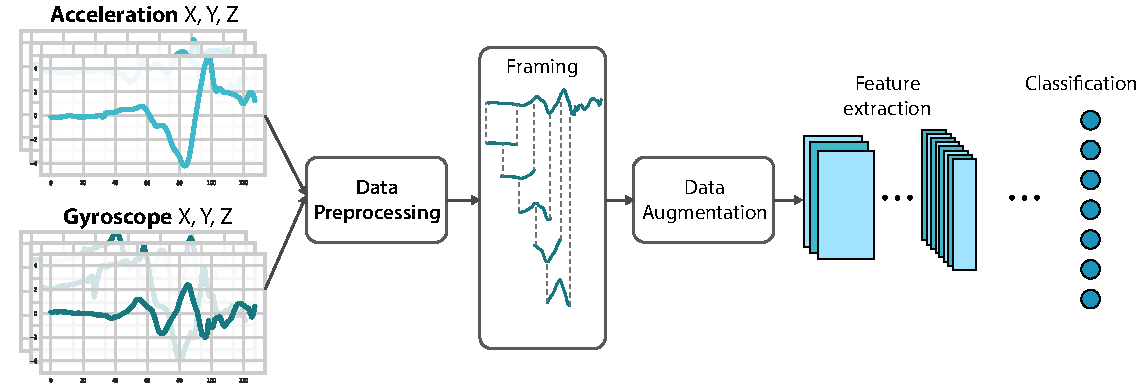
\includegraphics[width=\columnwidth]{pipeline}
    \caption{Schematic representation of the processing pipeline.}
    \label{fig:img_pipeline}
\end{figure}

Time series data from the IMU sensors is converted into contiguous segments through a \mbox{sliding-window} approach, the output of this process are feature vectors which represent the input of the machine learning models. Once the dataset is created, it is augmented and divided in training and test set and finally normalized. The basic blocks of all the approaches mentioned in this paper are the ones which typically constitute a CNN. Each CNN contains at least one convolution layer along the temporal domain, one pooling layer and at least one fully connected layer prior to a softmax layer. In the convolutional layer, a mathematical operation (i.e. convolution) applies a set of local filters (or kernels) to obtain the most representative features. After the convolution operation, a bias is added to the result. Subsequent \mbox{max-pooling} operations look for the maximum within a region of specific width and height, this corresponds to a subsampling which introduces translational invariance to the system and improves its robustness. The fully connected layer is applied at the end, combining all features' maps obtained by the previous convolutional steps and using it as input for a 7 neurons softmax layer which computes the probability of each activity class. Regularization techniques such as dropout, early stopping and partially, batch normalization, are used at different stages of the neural network in order to avoid overfitting to the training data. \par
Stacked denoising convolutional autoencoders (SDAs) are built on the same basic blocks mentioned above but follow a slightly different processing pipeline. \fig{fig:img_ae} represents the structure of a stacked autoencoder. The main building block is the autoencoder which can be separated into two parts, an encoder and a decoder. The encoder part consists of convolution layers and \mbox{fully-connected} layers and the decoder part consists of \mbox{fully-connected} layers and deconvolution layers. An ordinary autoencoder where the output $Y$ is of the same dimensionality as input $X$ can achieve perfect reconstruction simply by learning an identity mapping. This criterion alone is unlikely to lead to the discovery of a more useful representation of the input. The traditional approach to autoencoders uses a bottleneck to produce an \mbox{under-complete} representation, the resulting $Y$ can thus be seen as a lossy compressed representation of $X$. Since the reconstruction criterion alone is unable to guarantee the extraction of useful features, a more challenging and more interesting objective would be to clean a partially corrupted input (denoising). It's important to emphasize that the goal is not the task of denoising per se, rather denoising is investigated as a training criterion for learning to extract useful features that will constitute better higher level representation of the input \cite{Pascal-2010}. A key function of SDAs is unsupervised \mbox{pre-training}. Once each layer is \mbox{pre-trained} to conduct feature selection and extraction on the input from the preceding layer, a second stage of supervised \mbox{fine-tuning} can follow. The unsupervised \mbox{pre-training} of such architecture is done one layer at a time. Each layer is trained as a denoising autoencoder by minimizing the error in reconstructing its input. Once all layers are \mbox{pre-trained}, the network goes through a second stage of training known as supervised \mbox{fine-tuning} whose goal it to minimize prediction error on a supervised task. During this latter supervised phase only the dense layers are trained, while the rest is kept frozen.






\section{Signals and Features}
\label{sec:signals_features}

The dataset used in this paper is taken from \cite{base-paper} \footnote{The dataset is available at http://www.kn-s.dlr.de/activity/}. The IMU used provides the measurements in the sensor frame (SF) and the necessary attitude information in order to rotate them to the global frame (GF). However, acceleration and angular velocity relative to the human body seem to be the most relevant information (and not relative to an earth-fixed reference frame or the SF as the sensor can be placed on the body in any orientation and position) \cite{base-paper}.
The three axes of the body frame are defined to intersect at the sensor location, the z axis is directed towards the head, while the other axis (x and y) form the plane orthogonal to this vertical axis. The sensor was placed on the belt of the test candidates either on the right or the left part of the body.
As shown in \tab{activity_times_table} the final dataset contains over 5 hours of activity data. Class unbalance represents a major obstacle in the classification task. \\

\begin{table}[!htbp]
\captionsetup{font=scriptsize, justification=centering}
\centering
\resizebox{\columnwidth}{!}{%
\begin{tabular}{c|c|c|c|c|c|c|c|}
\cline{2-8}
\textbf{} & \textbf{Standing} & \textbf{Walking} & \textbf{Sitting} & \textbf{Lying} & \textbf{Running} & \textbf{Jumping} & \textbf{Falling} \\ \hline
\multicolumn{1}{|c|}{\textbf{Minutes}} & 121 & 72 & 59 & 28 & 15 & 8 & 2 \\ \hline
\end{tabular}%
}
\caption{Total activity data times for each recorded activity.}
\label{activity_times_table}
\end{table}

The original dataset contains the recordings of one IMU sensor:
\begin{itemize}
\item acceleration values along x, y, z axis
\item gyroscope values along x, y, z axis
\item attitude matrix to convert previous values from sensor to GF
\item magnetometer values along x, y, z axis
\end{itemize}
Each entry is either labeled with one of the activities among {\it running, jumping, walking, falling, sitting, standing, lying} or as a transition state between these base labels.

\subsection{Data preprocessing}
\label{sec:data_preprocessing}
The current classification task goal is to predict one of the base labels. Detecting transients was out of the scope of this paper and thus they were initially removed from the dataset. One mislabeling error was found and corrected, which was influencing just 5 frames in the original dataset.

\subsection{Framing}
\label{sec:framing}
After the initial preprocessing, the next step is to segment the \mbox{time-series} data into contiguous segments through a \mbox{sliding-window} approach (\fig{fig:img_framing}).\\

\begin{figure}[h]
	\captionsetup{font=scriptsize, justification=centering}
    \centering
	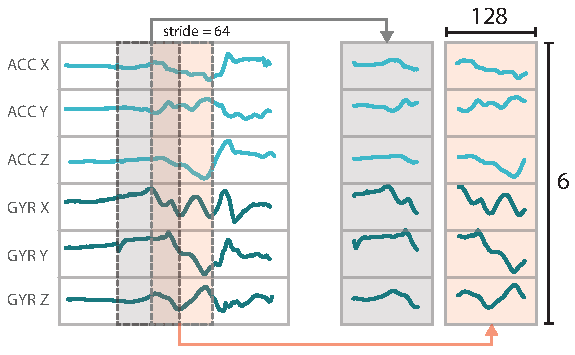
\includegraphics[width=\columnwidth]{framing}
    \caption{Framing procedure.}
    \label{fig:img_framing}
\end{figure}

Each frame or window will be then fed to the machine learning algorithm. Since 1sec is the minimal duration of an activity \cite{base-paper}, I used this as a reference for the window length. The sensor has a sampling rate of 100Hz, which means 100 \mbox{samples/sec}, so using a window length of 128 frames still captures the minimal duration of an activity, moreover it's the same value employed by \cite{base-paper}. The window is moved along the temporal domain progressively extracting samples that will generate the training and testing dataset. The step size of the sliding window is of 64 frames, so each window has 50\% overlapping with the previous one. Although this produces redundant data, it allows to generate a large number of samples, which is important for training a CNN. The label associated to each frame corresponds to the most frequent label of the 128 frames composing the window.
After windowing, the dataset is divided into training and test set following a \mbox{80/20} division, maintaining the class proportions in both test and training, as shown in \tab{test_train_prop_table}. Training set is composed of 22836 samples, test set of 5709 samples.

\begin{table}[!htbp]
\footnotesize
\captionsetup{font=scriptsize, justification=centering}
\centering
\begin{tabular}{r|c|c|c|}
\cline{2-4}
 & \textbf{Full} & \textbf{Test} & \textbf{Train} \\ \hline
\multicolumn{1}{|r|}{\textbf{Standing}} & 0.396532 & 0.396567 & 0.396523 \\ \hline
\multicolumn{1}{|r|}{\textbf{Walking}} & 0.236889 & 0.236819 & 0.236907 \\ \hline
\multicolumn{1}{|r|}{\textbf{Sitting}} & 0.193309 & 0.193204 & 0.193335 \\ \hline
\multicolumn{1}{|r|}{\textbf{Lying}} & 0.092626 & 0.092661 & 0.092617 \\ \hline
\multicolumn{1}{|r|}{\textbf{Running}} & 0.049361 & 0.049396 & 0.049352 \\ \hline
\multicolumn{1}{|r|}{\textbf{Jumping}} & 0.024838 & 0.024873 & 0.024829 \\ \hline
\multicolumn{1}{|r|}{\textbf{Falling}} & 0.006446 & 0.006481 & 0.006437 \\ \hline
\end{tabular}
\caption{Class proportions in full dataset compared to test and training set.}
\label{test_train_prop_table}
\end{table}

\subsection{Data augmentation}
\label{sec:data_augmentation}
Data augmentation is the practice of augmenting real IMU training data with simulated data for improving the recognition accuracy. Appropriate augmentation can substancially improve classification performance, especially in situations with small dataset size, noisy labels, and large \mbox{intra-class} variability \cite{terry-2017}. The latter being an especially known problem in HAR tasks \cite{Andreas-2014}. During the data augmentation process, the imbalance issue is tackled by creating a larger number of augmented samples for the under represented classes. The samples are \mbox{re-balanced} such that each class has at least 35\% percent of the largest number of samples per class in the training set.\\
In the field of computer vision, synthetic data (\mbox{computer-generated} data that mimics real data) is used used to augment or create training data for increasing classification performance \cite{xi-2015}.\\
As there exist many kinds of data augmentation techniques, the most promising from \cite{terry-2017} are implemented in this paper. Permutation is a simple way to randomly perturb the temporal location of \mbox{within-window} events. To perturb the location of the data in a single window, I first slice the data into 5 samelength segments, and randomly permute the segments to create a new window. Another factor that can introduce \mbox{label-invariant} variability of wearable sensor data are differences in sensor placement. For example, an \mbox{upside-down} placement of the sensor can invert the sign of the sensor readings without changing the labels. Therefore, augmentation by applying arbitrary rotations to the existing data can be used as a way of simulating different sensor placements. To achieve the \mbox{intra-class} balance mentioned before, the input vectors quantities summarised in \tab{augmentation_sizes_table} were generated by combining the two mentioned data augmentation approaches.

\begin{table}[!htbp]
\footnotesize
\captionsetup{font=scriptsize, justification=centering}
\centering
\begin{tabular}{r|c|c|
>{\columncolor[HTML]{E5E5E5}}c |}
\cline{2-4}
 & \textbf{Original size} & \textbf{Increment} & \textbf{Augmented size} \\ \hline
\multicolumn{1}{|r|}{\textbf{Standing}} & 9055 & 0 & 9055 \\ \hline
\multicolumn{1}{|r|}{\textbf{Walking}} & 5410 & 0 & 5410 \\ \hline
\multicolumn{1}{|r|}{\textbf{Sitting}} & 4415 & 0 & 4415 \\ \hline
\multicolumn{1}{|r|}{\textbf{Lying}} & 2115 & 1054 & 3169 \\ \hline
\multicolumn{1}{|r|}{\textbf{Running}} & 1127 & 2042 & 3169 \\ \hline
\multicolumn{1}{|r|}{\textbf{Jumping}} & 567 & 2602 & 3169 \\ \hline
\multicolumn{1}{|r|}{\textbf{Falling}} & 147 & 3022 & 3169 \\ \hline
\end{tabular}
\caption{Number of samples generated to augment the original dataset and representation of the new class balance in the augmented dataset.}
\label{augmentation_sizes_table}
\end{table}

Considering the conspicuous amount of data that was discarded when removing all the transients from the original dataset, specifically 1 hour of data, I tried an alternative data augmentation approach that leveraged this wealth of data. Transients are unlabeled frames that sit between two consecutive labeled activities. The idea of this approach is to assign specific labels to this transients according to the previous and following activity, specifically half of the frames of each transient was labeled as the preceding activity and the remaining half was labeled as the following activity. As a result of this data augmentation phase, I obtained 3 datasets: the original non-augmented, the augmented through rotation and permutation (\texttt{aug}) and another one with transitions converted to labels (\texttt{trans}).\\

Finally, the input data is normalized before it is fed into the feature extractor. I computed mean and standard deviation for each axis of the considered sensor values (acceleration and gyroscope) and normalized the input data by subtracting mean and dividing by the standard deviation. Both training and test set were normalized using the values computed on the training set, by doing this, no bias or additional information in introduced in the test set.


\section{Learning Framework}
\label{sec:learning_framework}

The neural networks here described are implemented in Keras, a lightweight library to build and train neural networks. The model training and classification are run on a {\it p2.xlarge} EC2 AWS instance which features Intel Xeon E5-2686 v4 (Broadwell) processor, 61GiB of ram and one NVIDIA K80 GPU. \\
The following sections describe in detail the topology and the parameters of the three basic machine learning models used to solve the HAR task tackled in this paper.
Sensor data are \mbox{re-organized} to be of shape \texttt{?x1x128x6} where 1 is the depth, 128 is the length of a sensor window and 6 is the number of sensor signals (acceleration x, y, z - gyroscope x, y, z). This format (known as "channel first" in Keras) was used for compatibility reasons with the GPU backend of Keras. All models are using mini-batch gradient descent (64 samples per batch) with RMSProp update rule with $ learningrate=0.001$ and $\rho=0.9$.

\subsection{CNN with only 1D temporal convolutions (\texttt{m_1d})}
\label{sec:m_1d}
This is the simplest of the architectures explored in this paper and involves only temporal convolutions, i.e. convolutions along the time domain. The topology of the model is described in detail in \tab{m_1d_table}

\begin{table}[!htbp]
\captionsetup{font=scriptsize, justification=centering}
\centering
\resizebox{\columnwidth}{!}{%
\begin{tabular}{|l|c|c|c|c|c|c|c|c|}
\hline
\multicolumn{1}{|c|}{\textbf{Input}} & \textbf{Conv} & \textbf{D.M.} & \textbf{Conv} & \textbf{D.M.} & \textbf{Flat} & \textbf{Dense} & \textbf{D} & \textbf{Softmax} \\ \hline
1@(6x128) & 30@(1x5) &  & 40@(1x5) &  &  & 150 &  & 7 \\ \hline
\end{tabular}%
}
\caption{\texttt{m_1d} model representation. Each \texttt{Conv} layer is made of (i) a convolution layer, (ii) a batch normalization and (iii) a ReLU activation. \texttt{D.M.} stands for dropout and max pooling, \texttt{D} stands for dropout. All dropout layers were set to 0.3 except the last one, set to 0.2.}
\label{m_1d_table}
\end{table}

Each conv section is constituted by (i) a convolution layer that convolves the input or the previous layer's output along the temporal domain with a set of kernels to be learned; (ii) a batch normalization along the time domain, (iii)  a rectified linear unit (ReLU) layer that maps the output of the previous layer by the function $ relu(v) = max(v; 0) $. Dropout layers set the activation of \mbox{randomly-selected} units during training to zero with probability 0.3 for the first two occurennces and 0.2 in the last dropout layer and this is added as a form of regularization. Max pooling is used to further reduce the dimensionality and increase the spatial invariance of features. After the convolutions, all the feature maps values of the previous layer are concatenated using a \mbox{fully-connected} layer (indicated as {\it Flat} in \tab{m_1d_table}). Following is a \mbox{fully-connected} layer with 150 neurons and lastly another \mbox{fully-connected} layer with $C=7$ neurons, where $C$ is the number of output classes.
The output of this layer is governed by the softmax function
$$ \sigma(z)_j = \frac{e^{z_j}}{\sum_{k=1}^{\kappa} e^{z_k}} $$
where $ \kappa $ is the total number of classes (7 in this case) and $ z_j $ represents the j-th entry of the score vector $ z $.
This softmax function provides the posterior probability of the classification results. Then, an entropy cost function can be constituted based on the true labels of training instances and probabilistic outputs of softmax function
$$ L(\theta) = -\frac{1}{n} \sum_{i=1}^{n} \sum_{j=1}^{m} y_{ij} log(p_{ij}) $$
where $i$ indexes samples, $j$ indexes classes and $y$ is the sample label (one-hot vector in multiclass classification), $p_{ij} \varepsilon (0,1)$ and $\sum_{j} p_{ij} = 1$ is the prediction for a sample.
The network parameters are optimized by minimizing the categorical cross-entropy loss function using mini-batch gradient descent with the RMSProp update rule. \\

\subsection{CNN with 2D convolutions (\texttt{m_2d})}
\label{sec:m_2d}
This model follows the same architecture as \texttt{m_1d}, but uses only 2D convolutions. Model specification are found on \tab{m_2d_table}

\begin{table}[!htbp]
\captionsetup{font=scriptsize, justification=centering}
\centering
\resizebox{\columnwidth}{!}{%
\begin{tabular}{|c|c|c|c|c|c|c|c|c|}
\hline
\textbf{Input} & \textbf{Conv} & \textbf{Conv} & \textbf{Conv{[}pad{]}} & \textbf{MP} & \textbf{Flat} & \textbf{Dense} & \textbf{D} & \textbf{Softmax} \\ \hline
1@(6x128) & 20@(2x4) & 40@(2x2) & 60@(4x4) &  &  & 150 & 0.3 & 7 \\ \hline
\end{tabular}%
}
\caption{\texttt{m_2d} model representation. Each \texttt{Conv} layer is made of (i) a convolution layer, (ii) a batch normalization, (iii) a ReLU activation and (iv) a Dropout set to 0.2. \texttt{pad} indicates that zero-padding is used, \texttt{D} stands for dropout, \texttt{MP} stands for max pooling.}
\label{m_2d_table}
\end{table}

\subsection{CNN with 1D and 2D convolutions (\texttt{m_1d2d_01})}
\label{sec:m_1d2d}
This model extends the previous ones by testing also the effect of cross correlating the signals of different sensors by using both 1D and 2D convolutions. The topology of this model is summarized in \tab{m_1d2d_table}

\begin{table*}[]
\captionsetup{font=scriptsize, justification=centering}
\centering
\resizebox{\textwidth}{!}{%
\begin{tabular}{|c|l|c|c|c|c|c|c|c|c|c|c|c|c|c|c|c|}
\hline
\textbf{Input} & \textbf{BN} & \textbf{Conv} & \textbf{Conv} & \textbf{D} & \textbf{Conv} & \textbf{Conv} & \textbf{D} & \textbf{MP} & \textbf{Conv} & \textbf{MP} & \textbf{Conv} & \textbf{D} & \textbf{Flat} & \textbf{Dense} & \textbf{D} & \textbf{Softmax} \\ \hline
1@(6x128) &  & 16@(1x4) & 32@(1x4) & 0.3 & 64@(1x3) & 64@(3x3) & 0.3 &  & 64@(3x2) &  & 64@(3x2) & 0.3 &  & 150 & 0.2 & 7 \\ \hline
\end{tabular}%
}
\caption{\texttt{m_1d2d_01} model representation. Each \texttt{Conv} layer is made of (i) a convolution layer and (ii) a ReLU activation, stride is set to (1x1). \texttt{BN} stands for batch normalization. \texttt{D} represents a dropout layer and the number beneath is the percentage of elements that will be set to zero. \texttt{MP} stands for max pooling. \texttt{Flat} concatenates all the feature map values of the previous layer. Dense is a fully connected layer. \texttt{X@($Y \times Z$)} indicates the number of kernels, $X$, and the size of the kernel matrix, $Y \times Z$.}
\label{m_1d2d_table}
\end{table*}

Keeping \tab{m_1d2d_table} as a reference, the first 3 convolutional blocks operate only temporal convolutions, starting from the 4th block, \mbox{cross-correlation} among input vectors is considered too. In these 2D convolutional layers, \mbox{zero-padding} is also applied in order to keep the $(Y \times Z)$ feature map dimension invariant during convolution operations, this was necessary in order to achieve a deeper network.\\

I tested two other different variations of this model, specifically:
\begin{itemize}
\item \texttt{m_1d2d_01_reg} which features the same topology, but L2 regularization was applied to the last 2 dense layers, in an attempt to prevent overfitting. L2 regularization adds a penalty parameter to the loss function, the value of the multiplier was set to $\lambda=0.001$, setting it to 0 reverts to the case of no normalization.
\item \texttt{m_1d2d} which instead of having a single batch normalization at the beginning, applies batch normalization layer after each convolution operation
\end{itemize}

\subsection{CNN with skip connections (\texttt{m_resnet})}
\label{sec:m_resnet}
The main benefit of a very deep network is that it can represent very complex functions. However, a huge barrier to training them is vanishing gradients: while backpropagating from the final layer back to the first layer, the weight matrix is multiplied on each step, and thus the gradient can decrease exponentially quickly to zero. Residual networks (ResNets) were first proposed by \cite{resnets-2015} and managed to build very deep CNNs by using skip connections (or shortcuts) to help the backpropagation of the gradient.
The basic building blocks of a ResNet are identity and convolutional shortcuts (\fig{fig:img_resnet}): identity shortcuts can be directly used when the input and output are of the same dimensions (\fig{fig:img_resnet} left). When the dimensions increase, projection shortcuts (\fig{fig:img_resnet} right) are used to match dimensions (done by $1 \times 1$ convolutions). \\

\begin{figure}[h]
	\captionsetup{font=scriptsize, justification=centering}
    \centering
	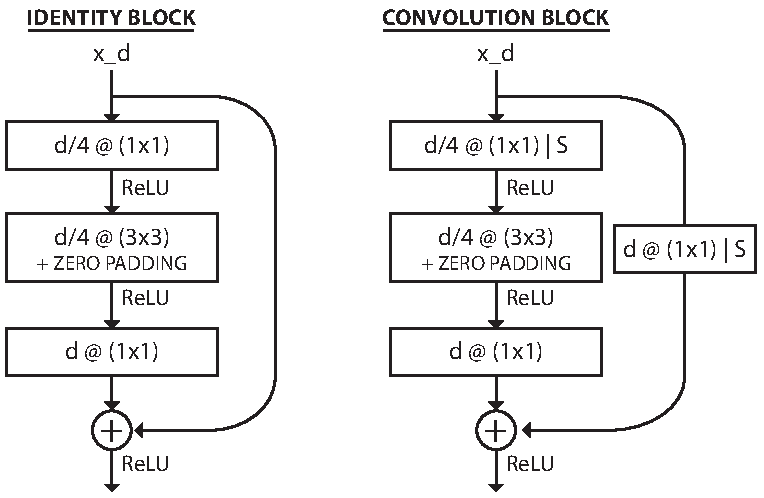
\includegraphics[width=\columnwidth]{resnet-blocks}
    \caption{Building blocks of a ResNet. Identity block is used when input and output dimension are the same, otherwise the convolution block is used. \texttt{x_d} indicates the input \texttt{x} of depth \texttt{d}. \texttt{| S} suffix indicates that a custom stride, different from $1 \times 1$ is applied to that convolution.}
    \label{fig:img_resnet}
\end{figure}

In this paper I implement {\it ResNet-50} and I suggest \cite{resnets-2015} for full details on the implementation.\\
This model is achieved by stacking groups of identity blocks and convolutional blocks to form a 50 layer deep network, the topology is described in \tab{m_resnet_table}.

\begin{table*}[]
\captionsetup{font=scriptsize, justification=centering}
\centering
\resizebox{\textwidth}{!}{%
\begin{tabular}{|c|c|c|c|c|c|c|c|c|c|c|c|}
\hline
\multicolumn{1}{|c|}{\textbf{Input}} & \textbf{Conv} & \textbf{BN} & \textbf{ReLU} & \textbf{MP} & \textbf{S1} & \textbf{S2} & \textbf{S3} & \textbf{S4} & \textbf{AP} & \textbf{Flat} & \textbf{Softmax} \\ \hline
1@(6x128) & 32@(1x4) &  &  &  & 
$\begin{bmatrix} 32@(1 \times 1) \\ 32@(3 \times 3) \\ 128@(1 \times 1) \end{bmatrix} \times 3$ &
$\begin{bmatrix} 64@(1 \times 1) \\ 64@(3 \times 3) \\ 256@(1 \times 1) \end{bmatrix} \times 4$ &
$\begin{bmatrix} 128@(1 \times 1) \\ 128@(3 \times 3) \\ 512@(1 \times 1) \end{bmatrix} \times 6$ &
$\begin{bmatrix} 256@(1 \times 1) \\ 256@(3 \times 3) \\ 1024@(1 \times 1) \end{bmatrix} \times 3$ &
1x2 &  & 7 \\ \hline
\end{tabular}%
}
\caption{\texttt{m_resnet} model representation. \texttt{BN} stands for batch normalization, \texttt{MP} for max pooling, \texttt{S1-S4} represent the 4 stages of the identity-convolutional blocks, the first block of every stage is convolutional, the rest are identity blocks. \texttt{AP} stands for average pooling, pooling is done only along the temporal dimension.}
\label{m_resnet_table}
\end{table*}

\subsection{Stacked denoising autoencoders (\texttt{m_ae})}
\label{sec:m_ae}
The main building block of this model is the autoencoder, an architecture composed of an encoder and a decoder. In this setup the autoencoders are composed only of convolutional layers and its topology is represented in \fig{fig:img_ae}. Lastly, the encoders are stacked together, followed by a \mbox{fully-connected} layer for the final classification.\\

\begin{figure*}[ht]
	\captionsetup{font=scriptsize, justification=centering}
    \centering
	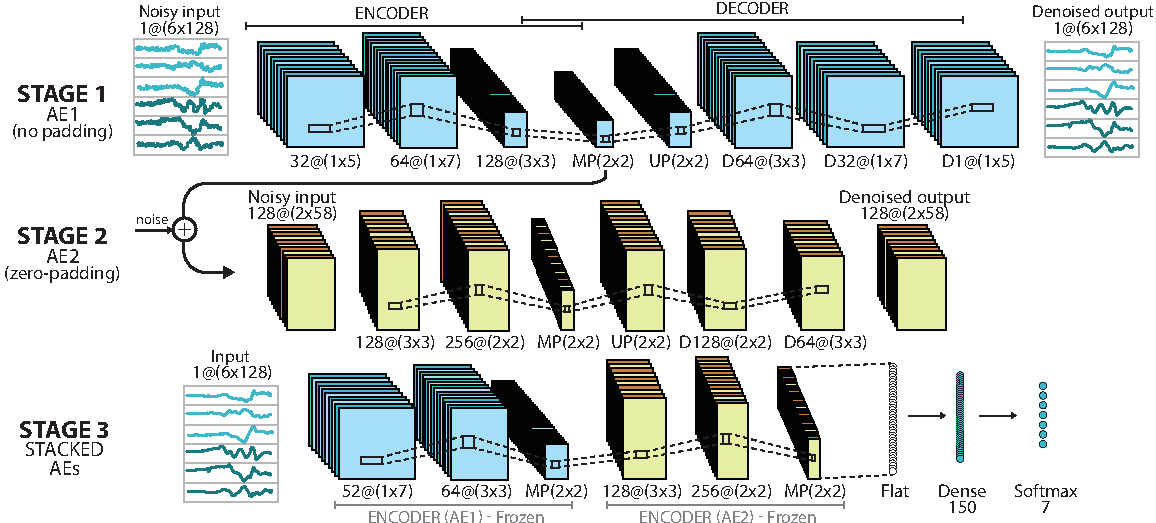
\includegraphics[width=\textwidth]{ae}
    \caption{Processing pipeline of a stacked denoising autoencoder. \texttt{MP} stands for max pooling, \texttt{UP} stands for up scaling, the opposite of a max pooling operation. Operations with \texttt{D} prefix stand for de-convolution operations, which revert the effect of a convolution. Zero-padding indicates that padding was used in convolution operations.}
    \label{fig:img_ae}
\end{figure*}

Training this kind of models follow a \mbox{two-step} procedure: (i) a corrupted input is used for the initial \mbox{denoising-training} of each individual layer, so that it may learn useful feature extractors. Once the mapping has been learnt, the output of the encoder part (with denoised data given as input) is used as input of the following autoencoder. Noise is always applied to the input of all the autoencoders during training. I tested with two different types of noise, as suggested by \cite{Pascal-2010}:

\begin{itemize}
\item Additive isotropic gaussian noise ($\mu = 0$, $\sigma=0.15$)
\item Masking noise, where a fraction of the elements of the input (chosen at random for each example) is set to 0
\end{itemize}

I also experimented with two different variations of the first autoencoder: this first one being represented in \fig{fig:img_ae} (\texttt{ae-long}) and another one that featured a shallower first autoencoder (\texttt{ae-short}), without an intermediate convolutional layer.

The network parameters of the autoencoders are optimized by minimizing the mean squared error loss function:
$$MSE = \frac{1}{n} \sum_{i=1}^{n}(y_i - \hat{y_i})^2$$

Once a stack of encoders has been trained, its output representation can be used as input to a \mbox{stand-alone} supervised learning algorithm. (ii) An output layer is added on top of the stack and the parameters of the whole system are \mbox{fine-tuned} to minimize the error in predicting the supervised target by performing gradient descent. It's important to note that during this \mbox{fine-tuning} phase the uncorrupted inputs are used and the layers of the stacked autoencoders are frozen i.e. no training is performed on these layers.

% !TEX root = template.tex

\section{Results}
\label{sec:results}

The evaluation of the models followed a progressive approach and the goal was twofold:
\begin{itemize}
\item find the best dataset i.e. augmented vs \mbox{non-augmented}
\item find the model with the best classification accuracy
\end{itemize}
In this paper I did not take into consideration the complexity of the model, so there was no constraints on the training or prediction time that would indeed have to be considered in the context of \mbox{real-time} prediction. \par

To evaluate the classification accuracy of the models I used the \mbox{F1-Score} parameter computed on a validation set, comprising 20\% of the total observations of the dataset. \mbox{F1-Score} is generally more appropriate then accuracy especially in cases of uneven class distribution, it is defined as the harmonic mean of precision and recall:

$$F_1 = 2 \cdot \frac{precision \cdot recall}{precision + recall}$$

Where precision is the ratio of correctly predicted positive observations to the total predicted positive observations.
$$Precision = \frac{TP}{TP+FP}$$
Recall is the ratio of correctly predicted positive observations to the all observations in true positive class.
$$Recall = \frac{TP}{TP+FN}$$

\subsection{Dataset results}
\label{sec:dataset_results}

To evaluate the dataset which offered the best classification accuracy, I tested the three datasets: (i) original, (ii) augmented with permutation and noise (\texttt{aug}) and (iii) augmented with replacement of the transition states (\texttt{trans}) with the following models: \texttt{m_1d}, \texttt{m_1d2d}, \texttt{m_1d2d_01}, \texttt{m_2d}. Refer to \secref{sec:learning_framework} for details on the model specifications and topology.\\

\tab{datasets_table} presents the \mbox{F1-Scores} for the aforementioned models and datasets.

\begin{table}[!htbp]
\captionsetup{font=scriptsize, justification=centering}
\centering
\resizebox{\columnwidth}{!}{%
\begin{tabular}{|r|c|c|c|c|c|c|c|c|c|c|c|c|}
\hline
 & \multicolumn{3}{c|}{\textbf{m\_1d}} & \multicolumn{3}{c|}{\textbf{m\_1d2d}} & \multicolumn{3}{c|}{\textbf{m\_1d2d\_01}} & \multicolumn{3}{c|}{\textbf{m\_2d}} \\ \hline
 & \textbf{std} & \textbf{trans} & \textbf{aug} & \textbf{std} & \textbf{trans} & \textbf{aug} & \textbf{std} & \textbf{trans} & \textbf{aug} & \textbf{std} & \textbf{trans} & \textbf{aug} \\ \hline
\textbf{Falling} & 0.757 & \cellcolor[HTML]{FFCE93}0.233 & \cellcolor[HTML]{9AFF99}0.773 & 0.794 & \cellcolor[HTML]{FFCE93}0.238 & \cellcolor[HTML]{9AFF99}0.882 & 0.8 & \cellcolor[HTML]{FFCE93}0.519 & \cellcolor[HTML]{9AFF99}0.879 & 0.794 & \cellcolor[HTML]{FFCE93}0.258 & \cellcolor[HTML]{9AFF99}0.838 \\ \hline
\textbf{Jumping} & 0.92 & \cellcolor[HTML]{FFCE93}0.584 & \cellcolor[HTML]{9AFF99}0.934 & 0.931 & \cellcolor[HTML]{FFCE93}0.587 & \cellcolor[HTML]{9AFF99}0.94 & 0.908 & \cellcolor[HTML]{FFCE93}0.538 & \cellcolor[HTML]{9AFF99}0.952 & 0.926 & \cellcolor[HTML]{FFCE93}0.598 & \cellcolor[HTML]{9AFF99}0.926 \\ \hline
\textbf{Lying} & 0.984 & \cellcolor[HTML]{FFCE93}0.919 & \cellcolor[HTML]{9AFF99}0.989 & 0.992 & \cellcolor[HTML]{FFCE93}0.935 & \cellcolor[HTML]{9AFF99}0.976 & 0.992 & \cellcolor[HTML]{FFCE93}0.927 & \cellcolor[HTML]{9AFF99}0.992 & 0.992 & \cellcolor[HTML]{FFCE93}0.919 & \cellcolor[HTML]{FFCE93}0.991 \\ \hline
\textbf{Running} & 0.972 & \cellcolor[HTML]{FFCE93}0.901 & \cellcolor[HTML]{9AFF99}0.981 & 0.989 & \cellcolor[HTML]{FFCE93}0.903 & \cellcolor[HTML]{9AFF99}0.995 & 0.986 & \cellcolor[HTML]{FFCE93}0.895 & \cellcolor[HTML]{9AFF99}0.998 & 0.988 & \cellcolor[HTML]{FFCE93}0.902 & \cellcolor[HTML]{9AFF99}0.991 \\ \hline
\textbf{Sitting} & 0.885 & \cellcolor[HTML]{FFCE93}0.785 & \cellcolor[HTML]{FFCE93}0.836 & 0.897 & \cellcolor[HTML]{FFCE93}0.839 & \cellcolor[HTML]{FFCE93}0.874 & 0.917 & \cellcolor[HTML]{FFCE93}0.874 & \cellcolor[HTML]{9AFF99}0.929 & 0.904 & \cellcolor[HTML]{FFCE93}0.825 & \cellcolor[HTML]{FFCE93}0.903 \\ \hline
\textbf{Standing} & 0.945 & \cellcolor[HTML]{FFCE93}0.845 & \cellcolor[HTML]{FFCE93}0.928 & 0.951 & \cellcolor[HTML]{FFCE93}0.86 & \cellcolor[HTML]{FFCE93}0.942 & 0.962 & \cellcolor[HTML]{FFCE93}0.888 & \cellcolor[HTML]{9AFF99}0.964 & 0.951 & \cellcolor[HTML]{FFCE93}0.858 & \cellcolor[HTML]{9AFF99}0.952 \\ \hline
\textbf{Walking} & 0.983 & \cellcolor[HTML]{FFCE93}0.915 & \cellcolor[HTML]{9AFF99}0.987 & 0.99 & \cellcolor[HTML]{FFCE93}0.906 & \cellcolor[HTML]{FFCE93}0.989 & 0.988 & \cellcolor[HTML]{FFCE93}0.933 & \cellcolor[HTML]{9AFF99}0.992 & 0.986 & \cellcolor[HTML]{FFCE93}0.915 & \cellcolor[HTML]{9AFF99}0.989 \\ \hline
\textbf{} & 0.945 & 0.836 & 0.932 & 0.954 & 0.851 & 0.945 & 0.961 & 0.878 & \textbf{0.967} & 0.954 & 0.849 & 0.955 \\ \hline
\end{tabular}%
}
\caption{F1-Scores of selected models with respect to three different datasets: (i) original \texttt{std}, (ii) augmented with permutation and noise (\texttt{aug}) and (iii) augmented with replacement of the transition states \texttt{trans}. Red cells indicate a degradation of the classification accuracy with respect to the standard dataset, green cells indicate an improvement. Best overall result is highlighted in bold.}
\label{datasets_table}
\end{table}

Before evaluating the impact of the different datasets, it's interesting to note that, as \cite{sensors-2018} suggested, the model \texttt{m_1d2d_01} with a single batch normalization layer performs better compared to its similar version, with multiple batch normalization layers (\texttt{m_1d2d}). Overall model with the best \mbox{F1-Score} among the ones in \tab{datasets_table} is \texttt{m_1d2d_01}, featuring both 1D and 2D convolutions, which achieves a \mbox{F1-Score} value of 0.967. Lets now consider the impact of different datasets: \texttt{trans} variation offers no improvement over the standard dataset, while the \texttt{augm} version consistently improve the classification accuracy with respect to the standard dataset. The major improvements are proportional to the augmentation entity of the underrepresented classes, specifically as can be seen from \tab{datasets_improvement_table} {\it falling} benefits from the biggest average increase accuracy and corresponds to the least represented class. Classes which had no augmentation received negligible variations with respect to the standard dataset.

\begin{table}[!htbp]
\footnotesize
\captionsetup{font=scriptsize, justification=centering}
\centering
\begin{tabular}{|r|c|c|}
\hline
 & \textbf{Augmentation entity} & \textbf{Mean improvement} \\ \hline
\textbf{Falling} & 3022 & 0.046 \\ \hline
\textbf{Jumping} & 2602 & 0.019 \\ \hline
\textbf{Running} & 2042 & 0.008 \\ \hline
\textbf{Lying} & 1054 & 0.001 \\ \hline
\textbf{Sitting} & 0 & -0.01 \\ \hline
\textbf{Standing} & 0 & 0 \\ \hline
\textbf{Walking} & 0 & 0.004 \\ \hline
\end{tabular}
\caption{Mean F1-Score improvement for all models of \tab{datasets_table} referred to the dataset augmented with permutation and noise \texttt{aug} with respect to the standard dataset. Augmentation entity represents the number of observations added to specific classes.}
\label{datasets_improvement_table}
\end{table}

It is thus reasonable to assume that the \texttt{aug} dataset improves the overall classification accuracy and will be the default dataset considered for tests on the subsequent models.

\subsection{Autoencoder results}
\label{sec:autoencoder_results}
Autoencoders were trained using the \texttt{aug} dataset. As mentioned in \secref{sec:m_ae}, four different variations are considered:
\begin{itemize}
\item \texttt{ae-long-gaus} represented in \fig{fig:img_ae} and whose inputs are corrupted using gaussian noise
\item \texttt{ae-long-zero} represented in \fig{fig:img_ae} and whose inputs are corrupted using zero masking
\item \texttt{ae-short-gaus} which is the shallower version of model in \fig{fig:img_ae} and whose inputs are corrupted using gaussian noise
\item \texttt{ae-short-zero} which is the shallower version of model in \fig{fig:img_ae} and whose inputs are corrupted using zero masking
\end{itemize}

A qualitative assessment of the reconstruction accuracy of the autoencoder can be seen in \fig{fig:img_signal_reconstruction}. The model seems to be able to remove noise pretty effectively and the rebuilt signal overlaps most of the times with the original uncorrupted input. \\

\begin{figure}[h]
	\captionsetup{font=scriptsize, justification=centering}
    \centering
	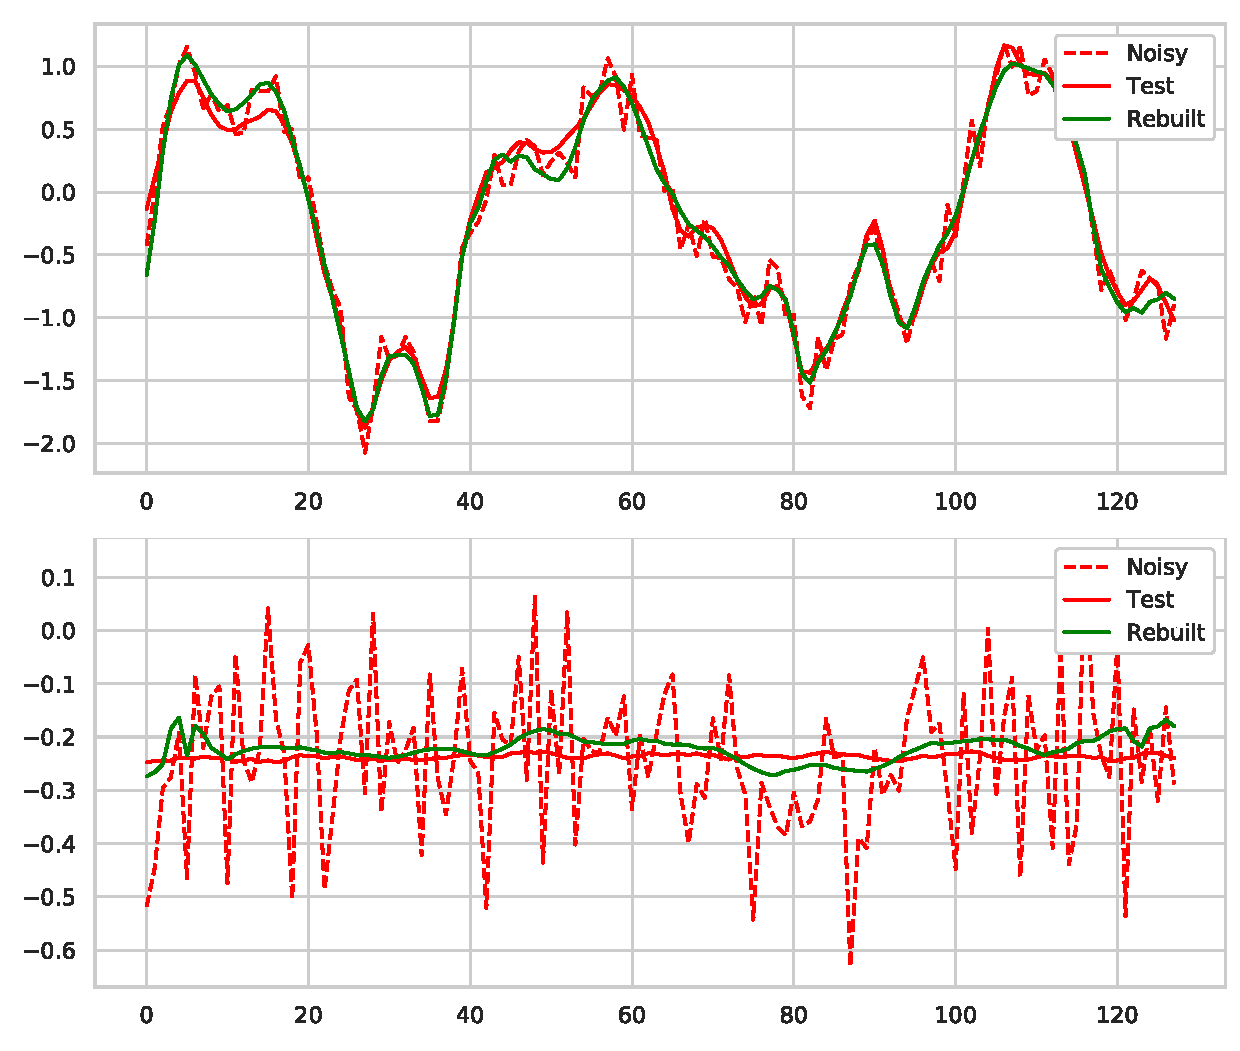
\includegraphics[width=\columnwidth]{ae-signals}
    \caption{Reconstruction of some sample signals done by the first autoencoder of the \texttt{ae-long} model. {\it Noisy} is the noisy input used for training, {\it Test} is the orinal uncorrupted signal, {\it Rebuilt} is the reconstructed signal by the trained autoencoder.}
    \label{fig:img_signal_reconstruction}
\end{figure}

\tab{ae_comparison_table} Compares the different stacked autoencoders \mbox{F1-Scores}.

\begin{table}[!htbp]
\footnotesize
\captionsetup{font=scriptsize, justification=centering}
\centering
\resizebox{\columnwidth}{!}{%
\begin{tabular}{|r|c|c|c|c|}
\hline
\multicolumn{1}{|c|}{} & \textbf{ae-long-gaus} & \textbf{ae-long-zero} & \textbf{ae-short-gaus} & \textbf{ae-short-zero} \\ \hline
\textbf{Falling} & 0.667 & 0.571 & \textbf{0.720} & 0.656 \\ \hline
\textbf{Jumping} & 0.838 & 0.805 & \textbf{0.849} & 0.766 \\ \hline
\textbf{Lying} & \textbf{0.985} & 0.985 & 0.985 & 0.985 \\ \hline
\textbf{Running} & \textbf{0.956} & 0.945 & 0.947 & 0.949 \\ \hline
\textbf{Sitting} & \textbf{0.867} & 0.823 & 0.850 & 0.847 \\ \hline
\textbf{Standing} & \textbf{0.935} & 0.912 & 0.926 & 0.920 \\ \hline
\textbf{Walking} & \textbf{0.979} & 0.965 & 0.972 & 0.975 \\ \hline
\rowcolor[HTML]{E1E1E1} 
\textbf{Mean} & \textbf{0.934} & 0.911 & 0.925 & 0.921 \\ \hline
\end{tabular}%
}
\caption{F1-Scores for various stacked autoencoders, \texttt{long} prefix indicates the deeper version of the first autoencoder, as presented in \secref{sec:m_ae}, \texttt{short} prefix indicates the shallower version. \texttt{gaus} suffix indicates the model trained with inputs corrupted by gaussian noise, \texttt{zero} instead indicates input corruption with zero-masking.}
\label{ae_comparison_table}
\end{table}

While the best \mbox{F1-Score} is achieved by \texttt{long-gaus} model with a value of 0.934, just 0.009 improve with respect to the shallower version, the shallow version was able to achieve a better classification accuracy on underrepresented classes. The deeper version was probably able to build a more complex representation of the input data for classes with a higher number of samples, thus offering an improved \mbox{F1-Score} on specific classes i.e. {\it running, sitting, standing, walking}. Lastly, the autoencoder with gaussian noise performed slightly better compared to the zero-masking one.

\subsection{Overall model comparison}
\label{sec:final_results}
The previous two sections were aimed to find the best version of the analysed models in order to perform additional fine tunings and thus do a final comparison with the remaining model, which is presented in this section.\\
In this section two more models are introduced:
\begin{itemize}
\item \texttt{m_1d2d_01_reg} which has the same topology as \texttt{m_1d2d_01} but adds L2 regularization in the last 2 dense layers
\item \texttt{m_resnet} which is {\it ResNet-50}
\end{itemize}

The models were compared using the \texttt{aug} dataset and the \mbox{F1-scores} are summarized in \tab{final_models_table}.

\begin{table}[!htbp]
\captionsetup{font=scriptsize, justification=centering}
\centering
\resizebox{\columnwidth}{!}{%
\begin{tabular}{r|c|c|c|c|c|c|c|}
\cline{2-8}
 & \textbf{ae-long-gaus} & \textbf{m\_3d} & \textbf{m\_1d2d\_01} & \textbf{m\_1d2d\_01\_reg} & \textbf{m\_1d2d} & \textbf{m\_1d} & \textbf{m\_resnet} \\ \hline
\multicolumn{1}{|r|}{Falling} & 0.667 & 0.838 & 0.879 & \textbf{0.919} & 0.882 & 0.773 & 0.872 \\ \hline
\multicolumn{1}{|r|}{Jumping} & 0.838 & 0.926 & 0.952 & \textbf{0.964} & 0.94 & 0.934 & 0.936 \\ \hline
\multicolumn{1}{|r|}{Lying} & 0.985 & 0.991 & 0.992 & \textbf{0.993} & 0.976 & 0.989 & 0.992 \\ \hline
\multicolumn{1}{|r|}{Running} & 0.956 & 0.991 & 0.998 & \textbf{0.998} & 0.995 & 0.981 & 0.989 \\ \hline
\multicolumn{1}{|r|}{Sitting} & 0.867 & 0.903 & 0.929 & \textbf{0.94} & 0.874 & 0.836 & 0.92 \\ \hline
\multicolumn{1}{|r|}{Standing} & 0.935 & 0.952 & 0.964 & \textbf{0.969} & 0.942 & 0.928 & 0.956 \\ \hline
\multicolumn{1}{|r|}{Walking} & 0.979 & 0.989 & 0.992 & \textbf{0.992} & 0.989 & 0.987 & 0.99 \\ \hline
\rowcolor[HTML]{D9D9D9} 
\multicolumn{1}{|r|}{\cellcolor[HTML]{D9D9D9}Mean} & 0.934 & 0.955 & 0.967 & \textbf{0.972} & 0.945 & 0.932 & 0.961 \\ \hline
\end{tabular}%
}
\caption{F1-Scores of selected models.}
\label{final_models_table}
\end{table}

Training curves of the experiments are depicted in \fig{fig:img_f1_scores}\\

\begin{figure}[h]
	\captionsetup{font=scriptsize, justification=centering}
    \centering
	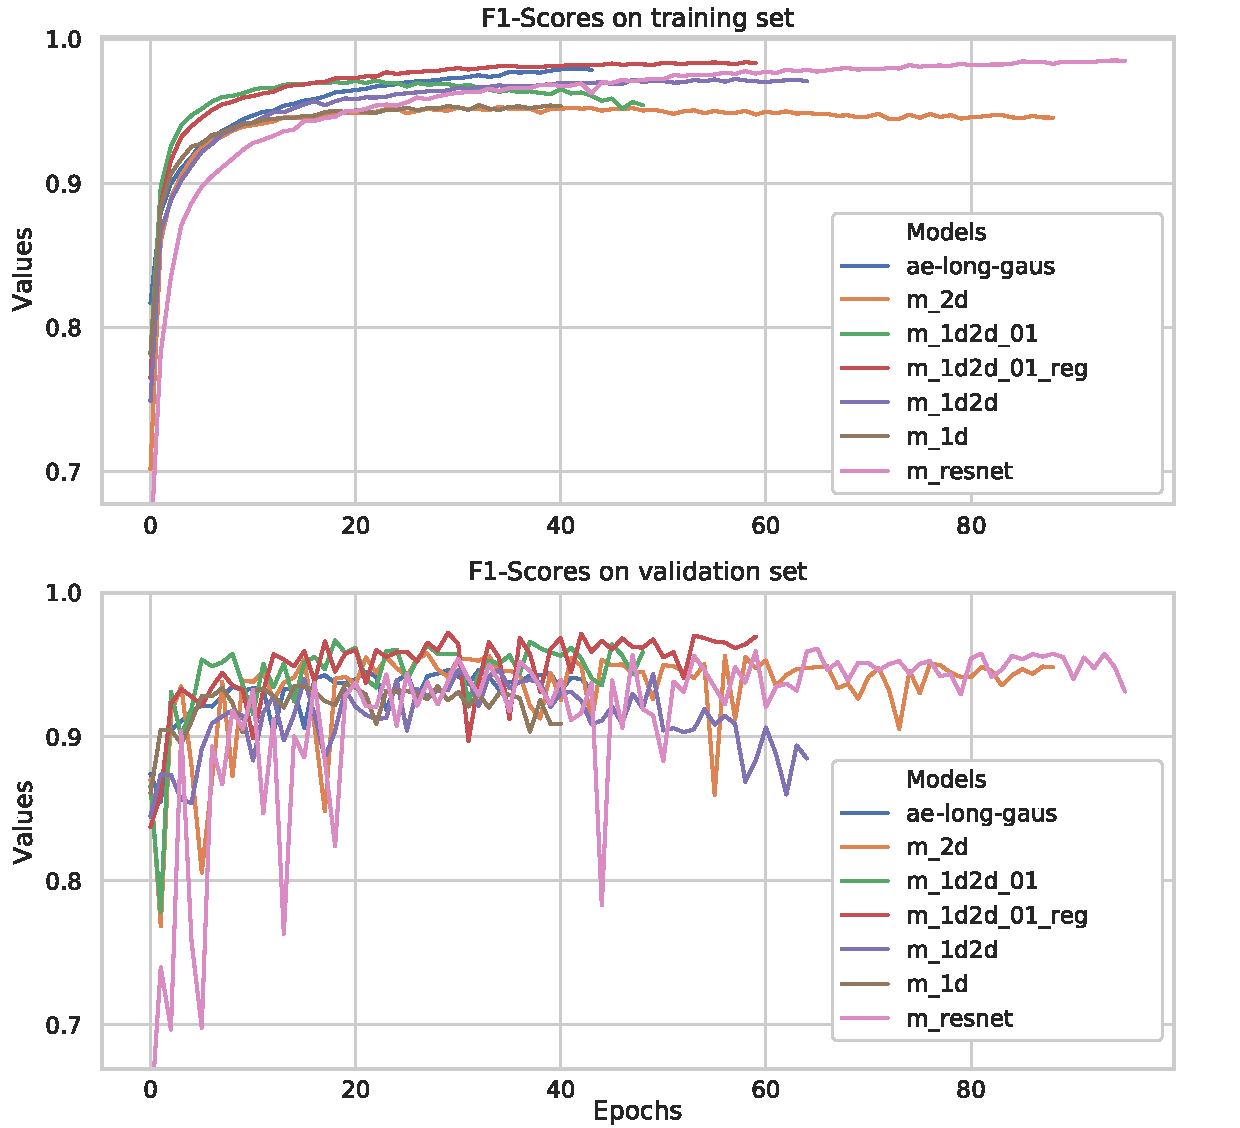
\includegraphics[width=\columnwidth]{f1-scores}
    \caption{F1-Scores for training and validation set.}
    \label{fig:img_f1_scores}
\end{figure}

The regularized version of model \texttt{m_1d2d_01} was able to remove the overfitting problem which is very visibile at approximately 20 epochs (\fig{fig:img_f1_scores}) and was thus be able to improve its classification accuracy. Batch size and the learning rate may be influencing the fluctuations in the validation accuracy plot of \fig{fig:img_f1_scores}.\\
Overall the best model achieves an \mbox{F1-Score} of 0.972 and the confusion matrix related to this model is presented in \tab{conf_matrix}

\begin{table}[!htbp]
\captionsetup{font=scriptsize, justification=centering}
\centering
\resizebox{\columnwidth}{!}{%
\begin{tabular}{cc|c|c|c|c|c|c|c|c|}
\cline{3-10}
 &  & \multicolumn{7}{c|}{\cellcolor[HTML]{B2B2B2}\textbf{Predicted}} & \cellcolor[HTML]{E5DFDF} \\ \cline{3-9}
 &  & Falling & Jumping & Lying & Running & Sitting & Standing & Walking & \multirow{-2}{*}{\cellcolor[HTML]{E5DFDF}\textbf{Recall}} \\ \hline
\multicolumn{1}{|c|}{\cellcolor[HTML]{B2B2B2}} & Falling & \textbf{0.92} & 0 & 0.027 & 0 & 0.054 & 0 & 0 & 0.919 \\ \cline{2-10} 
\multicolumn{1}{|c|}{\cellcolor[HTML]{B2B2B2}} & Jumping & 0 & \textbf{0.93} & 0 & 0.007 & 0 & 0.021 & 0.042 & 0.930 \\ \cline{2-10} 
\multicolumn{1}{|c|}{\cellcolor[HTML]{B2B2B2}} & Lying & 0.0057 & 0 & \textbf{0.99} & 0 & 0.0057 & 0 & 0 & 0.989 \\ \cline{2-10} 
\multicolumn{1}{|c|}{\cellcolor[HTML]{B2B2B2}} & Running & 0 & 0 & 0 & \textbf{1} & 0 & 0 & 0 & 1 \\ \cline{2-10} 
\multicolumn{1}{|c|}{\cellcolor[HTML]{B2B2B2}} & Sitting & 0 & 0 & 0 & 0 & \textbf{0.92} & 0.083 & 0 & 0.917 \\ \cline{2-10} 
\multicolumn{1}{|c|}{\cellcolor[HTML]{B2B2B2}} & Standing & 0 & 0 & 0 & 0 & 0.015 & \textbf{0.98} & 0.0013 & 0.984 \\ \cline{2-10} 
\multicolumn{1}{|c|}{\multirow{-7}{*}{\cellcolor[HTML]{B2B2B2}\textbf{True}}} & Walking & 0 & 0 & 0 & 0 & 0 & 0.0096 & \textbf{0.99} & 0.990 \\ \hline
\multicolumn{2}{|c|}{\cellcolor[HTML]{E5DFDF}\textbf{Precision}} & 0.919 & 1 & 0.998 & 0.996 & 0.964 & 0.954 & 0.993 & \textbf{0.972} \\ \hline
\end{tabular}%
}
\caption{Confusion matrix of model \texttt{m_1d2d_01_reg} referred to the \texttt{aug} dataset}
\label{conf_matrix}
\end{table}

As a comparison with the reference paper \cite{base-paper}, \tab{comparison_table} reports the \mbox{F1-Scores} for the best model of this paper and the best model of \cite{base-paper}

\begin{table}[!htbp]
\footnotesize
\captionsetup{font=scriptsize, justification=centering}
\centering
\begin{tabular}{r|c|c|c|}
\cline{2-4}
\multicolumn{1}{c|}{} & \textbf{Reference} & \textbf{m\_1d2d\_01\_aug} & \textbf{Diff} \\ \hline
\multicolumn{1}{|r|}{\textbf{Falling}} & 0.889 & 0.919 & \cellcolor[HTML]{9AFF99}0.03 \\ \hline
\multicolumn{1}{|r|}{\textbf{Jumping}} & 0.930 & 0.964 & \cellcolor[HTML]{9AFF99}0.034 \\ \hline
\multicolumn{1}{|r|}{\textbf{Lying}} & 0.989 & 0.993 & \cellcolor[HTML]{9AFF99}0.004 \\ \hline
\multicolumn{1}{|r|}{\textbf{Running}} & 0.963 & 0.998 & \cellcolor[HTML]{9AFF99}0.035 \\ \hline
\multicolumn{1}{|r|}{\textbf{Sitting}} & 0.984 & 0.940 & \cellcolor[HTML]{FFCE93}-0.044 \\ \hline
\multicolumn{1}{|r|}{\textbf{Standing}} & 0.989 & 0.969 & \cellcolor[HTML]{FFCE93}-0.02 \\ \hline
\multicolumn{1}{|r|}{\textbf{Walking}} & 0.989 & 0.992 & \cellcolor[HTML]{9AFF99}0.003 \\ \hline
\end{tabular}
\caption{F1-Scores of best model of reference paper \cite{base-paper} vs the best model of this paper along with the difference between the two approaches.}
\label{comparison_table}
\end{table}

% !TEX root = template.tex

\section{Concluding Remarks}
\label{sec:conclusions}
In this paper I explored the performance of various deep learning approaches based on CNNs for HAR using a single wearable sensor. The goal was to improve the result of \cite{base-paper} and prove that automatic feature extration would result in high classification accuracy. This task was successfully tackled using a 8-layer CNN and the proposed data augmentation methods. The combination of rotational and permutational data augmentation methods improves the baseline \mbox{F1-Score} of 0.961 to 0.967, overall improvement is not substancial but specific underrepresented classes received most benefit.
By comparing CNNs with 1D (temporal-only) convolutions, CNNs with both 1D and 2D convolutions, ResNets and stacked denoising autoencoders, the best model was a 8-layer CNN with both 1D and 2D convolutions capturing also the cross-correlation between different sensor values. I managed to achieve an \mbox{F1-Score} of 0.972 on the best performing model.
Many recent research papers as \cite{nils-2016, Valarezo-2017, su-2016} show that recurrent neural networks consistenly outperform deep neural networks and CNNs in HAR tasks and this would definitely be an interesting architecture to test against the ones developed in this paper. I did not experiment with different sampling rates, which is a crucial topic when dealing with wearable devices: reduced sampling rates imply more efficient resource use in \mbox{real-world} deployments. Minimal changes in the model architecture may result in noticeable improvement in the classification accuracy, as I showed in \secref{sec:final_results}. Random exploration of the parameter space for each model would be an effective strategy to iteratively \mbox{fine-tune} selected models as shown by \cite{nils-2016}.
Moreover, aside from the technical challenges I had to overcome to develop this project, I realised the importance of reading and undestanding research material on the topic of interest, specifically machine learning applied to HAR tasks. Coming up with effective models requires both a deep understanding of machine learning and a background knowledge of HAR. Recent research papers are a great starting point to be aware of the state of the art architectures for the topic one's working on. This awareness gave me the motivation to write a clear, concise and understandable research paper and to open source my work at https://github.com/damnko/har-convolutional-neural-networks so that hopefully my effort can help the community.
As a last thing, this was my first opportunity to realise the importance of being confident in working with datasets and coming up with creative solutions to rearrange and elaborate data. The data preprocessing pipeline is as important as developing and testing the model and may require a substancial investment of time.

\bibliography{biblio}
\bibliographystyle{ieeetr}

\end{document}


